\documentclass[conference]{IEEEtran}
\IEEEoverridecommandlockouts
% The preceding line is only needed to identify funding in the first footnote. If that is unneeded, please comment it out.
\usepackage{cite}
\usepackage{amsmath,amssymb,amsfonts}
\usepackage{algorithmic}
\usepackage{graphicx}
\usepackage{textcomp}
\usepackage{xcolor}
\usepackage{tabularx} 
\usepackage{booktabs}
\usepackage{array}  
\def\BibTeX{{\rm B\kern-.05em{\sc i\kern-.025em b}\kern-.08em
    T\kern-.1667em\lower.7ex\hbox{E}\kern-.125emX}}

\title{Utilising Virtual Reality to Enhance Learning Outcomes in Basic Programming: A Study on Engagement and Conceptual Understanding}

\author{
    \IEEEauthorblockN{Jake Scerri}
    \IEEEauthorblockA{
        Institute of Information \& Communication Technology \\
        Malta College of Arts, Science \& Technology \\
        Corradino Hill, Paola PLA 9032 \\
        150704L, BSc (Hons) Multimedia Software Development \\
        Level 6, Year 3 \\
        jake.scerri.f32100@mcast.edu.mt
    }
}

\begin{document}

\maketitle

\begin{abstract}
This study investigates the use of Virtual Reality (VR) in programming education, with a focus on improving learner engagement and comprehension. The hypothesis proposed is that students learning basic programming in a virtual environment will exhibit higherlevels of engagement and understanding compared to those taught using traditional methods. The research applies a mixed methods approach to collect both qualitative and quantitative data. The aim is to offer a more effective and engaging way to teach programming to beginners through immersive virtual classroom simulations.
\end{abstract}

\begin{IEEEkeywords}
Virtual Reality, Programming Education, Engagement, Game-Based Learning, Educational Technology
\end{IEEEkeywords}

\section{Introduction, Positioning, and Research Onion}

\subsection{Description of Theme and Topic Rationale}
This study proposes investigating the integration of Virtual Reality into programming education with the intention of addressing common challenges in the classroom. Learners often face difficulty maintaining attention and comprehending abstract programming concepts. The intended project aims to utilise VR technology and gamification to enhance motivation, active engagement, and knowledge retention. Prior studies support the efficacy of interactive learning environments in improving educational outcomes.

\subsection{Positioning and Research Onion}
This research is situated within the intersecting domains of education and technological innovation, particularly programming pedagogy.

\begin{itemize}
    \item \textbf{Philosophy:} A blend of qualitative and quantitative philosophies to ensure both perspectives are captured.
    \item \textbf{Approach:} Deductive logic is applied, informed by existing theories on game-based learning and VR.
    \item \textbf{Strategy:} Empirical research utilising both observational studies and semi-structured interviews.
    \item \textbf{Methods:} Mixed methods involving both statistical testing and thematic analysis of feedback and test scores.
\end{itemize}

\subsection{Background to This Research Theme}
Conventional programming instruction is often static and fails to maintain learners’ interest. Research has shown that VR and gamification positively influence student motivation and understanding. For instance, Hlavatý et al.[1] demonstrated how Unity-based educational games increase engagement. Theethum et al. [2] reported a 40.8\% improvement in comprehension using a VR game. López-Fernández et al. [3] also found that game-based methods consistently outperformed traditional approaches in engagement and memory retention.

\subsection{Hypothesis}
Students learning basic programming in a virtual reality environment will exhibit higher levels of engagement compared to those using traditional teaching methods.

\subsection{Research Aim and Purpose Statement}
\textbf{Aim:} To investigate how virtual reality enhances engagement, comprehension, and retention in basic programming education compared to traditional methods.\\
\textbf{Purpose:} To provide educators with innovative tools to improve outcomes in programming education, making the learning process more interactive, effective, and enjoyable.

\section{Literature Review}
Most VR application studies in programming instruction utilize quasi-experimental designs. As indicated in the study by Theethum et al. [2], who created the educational VR game Thinkercise, such studies normally utilise pre- and post-testing to quantify outcomes. In extending from this by including immersive self-avatar experiences and exploring computational thinking gains for middle school students, Parmar et al. [4] added to this. While Lopez-Fernandez et al. [3] employed a mixed-method approach that combined quantitative tests with qualitative semi-structured interviews to measure motivational impacts in game-based learning environments, Bicalho et al. [5] did a systematic review of the more general impact of VR on education. 
Academic and non-academic material must be separated from one another. Academic literature, including conference proceedings and peer-reviewed journal publications, report outcomes that have been rigorously evaluated (e.g., research papers published in IEEE journals) [6]. Non-academic sources, including prototype feedback reports and informal interviews, report useful information but are not peer reviewed, thus are to be used cautiously [7]. 
The following five peer-reviewed articles are suggested to support this study: (1) Thinkercise by Theethum et al. [2], (3) Game-Based Learning study by Lopez-Fernandez et al. [3], (4) VR Self-Avatar study by Parmar et al. [4], (5) Immersive VR Educational Practices by Bicalho et al. [5], and (6) Gamification for intrinsic motivation by Luarn et al. [8]. 
VR has been referred to in the literature as a revolutionary tool for transcending the conventional education challenges. The traditional lecture format cannot match the interactive, embodied learning experience of virtual reality. While [2] and [4] documented knowledge and participation increases, [3] observed an increase in motivation, but that knowledge acquisition may not differ significantly between the traditional learning method and game-based learning methods. As far as the issues of scalability and long-term retention of the programming knowledge acquired via VR interventions go, there is still an important gap. 
Since numerous studies are backing each of the concepts, a map of literature connecting VR in computer programming education can represent the interconnection between motivation, interest, and knowledge retention and how all the relationships are clear and properly labelled. 

\begin{figure}[htbp]
    \centering
    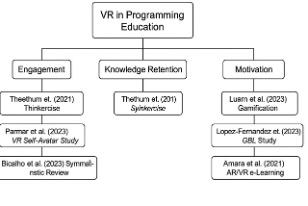
\includegraphics[width=\linewidth]{LiteratureMap.jpg}
    \caption{Literature Map on VR in Programming Education}
    \label{fig:literaturemap}
\end{figure}

\section{Research Methodology}
The primary research questions of this study are: (1) How does virtual reality influence students' engagement as compared to conventional methods? (2) How does virtual reality impact the comprehension and application of programming concepts? (3) Does virtual reality help people recall programming concepts eventually? 
The aims are to create an educational model of VR that can be applied to the students' learning requirements, compare their learning and retention levels through pre- and post-testing, and gain qualitative evidence from behaviour observation and semi-structured interviews. Choosing methodology was limited by an initial awareness of research paradigms and philosophies. The research is practical and honours both objective and subjective understanding. It is favourably disposed to positivist paradigms of analysis of measurable outcomes and paradigms for illuminating human understanding. 
A quasi-experimental design with mixed approaches was adopted. For the measurement of notable change, quantitative components review pre- and post-test measurement through paired samples t-tests [8]. Semi-structured interviews and observation are some of the qualitative aspects that provide greater insight into the experiences and likes of the users. In experimental design, one group of students will be initially taught in the conventional manner through PowerPoint presentations and will be given a pre-test. They will then be given a VR lesson; with the VR game questions incorporated into the post-test. To guarantee consistency, pre- and post-tests are administered to both groups. Additional qualitative data are gathered from follow-up interviews and session observation. Statistical and thematic analysis techniques will be utilized to examine the data. 
Use of tests, interviews, and observation augments the validity of this research. Having assessed the VR prototype before applying it ensures technical problems can be highlighted and addressed, thus increasing reliability. However, the small sample size and certain context of Level 3 program students limit generalisability. 
Gaining informed consent, protecting participant anonymity by using random user IDs, offering withdrawal, and keeping VR sessions short (ten minutes) to prevent physical discomfort are all ethical concerns. Additionally, participant feedback will be integrated to enhance the usability and accessibility of the VR application. 

\section{Project Implementation}

For this study to be carried out, the original plan of developing a Virtual Reality (VR) application was implemented, outlining different Python programming topics in immersive 3D environments. The application employed an enviroment, focused on delivering an immersive game experience while outlining fundamental concept in Python. this enviroment was split into different section, each section in the VR environment took about one minute to complete. The design emphasised Python variables and loops, which are essential yet often difficult for beginners to grasp. These core elements were chosen due to their foundational role in programming logic and problem-solving. All VR assets were sourced from online libraries, and the application was deployed using a Unity-based VR platform.

\subsubsection{Section 1 - Integer Variables}
In this VR scenario, users interact with a UI behind a table, where on pressing a button, this spawns triangles and increments an integer triangle counter variable. This incrementation process is shown, step by step, with arrows and highlighted code to show the code flow, and how is produces the output seen.

\subsubsection{Integer and Float Variable - Integration of both variables in a small game}
This section simulates a float variable, being decremented by 0.5 to simulate a timer running out. While the timer runs out, a user is presented with an empty bucket and with 3 shapes. He must throw the shapes in the bucket before the timer runs out! For every shape inserted in the bucket, a counter is incremented, with the appropriate code for both variables to show there workflow.

\subsubsection{Boolean Variables - Simple red light green light scenario}
The user is presented with a lever, that when he interacts with it, a light is switched from green to red, depending on the boolean variable value. 

\subsubsection{String Variables - Shape selection}
When a shape is picked up by the user, a String variable named ShapeName changes its value depending on the name of the shape.

\subsubsection{For and While Loops Scenario}
Shapes are spawned till a requirement is met or a value is changed. Code is being shown updating in real-time to show the loop behavior.

\subsubsection{Post-testing}
The user is then presented with questions, used a post-test questions, in the application it self. 

Throughout all VR sessions, interactive code was dynamically visualized, allowing users to directly link physical actions to logical programming constructs. The VR application was hosted and made available online.

\section{Evaluation Methodology}

Pre-test and post-test examinations were administered via Google Forms and comprised seven multiple-choice questions related to Python fundamentals. 54 MCAST Level 3 C\# programming students participated. Though familiar with programming, these students had limited exposure to Python and no prior experience with VR learning environments.

Four separate sessions were conducted: two using traditional video-based instruction and two using the custom VR application. All sessions began with a short introductory PowerPoint on Python basics, followed by a pre-test. The control group watched a seven-minute educational video, while the experimental group interacted with the VR application. A post-test followed each session.

The video and VR content were aligned to cover identical topics, ensuring parity in content exposure. Observers documented student engagement, focus levels, and interaction patterns throughout the sessions. Data from assessments were stored in Excel and analysed using SPSS to determine statistical significance in performance and behavioral differences.

\section{Findings and Discussion of Results}

\subsection{Results}

Independent and Paired Sample T-Tests were conducted. Each test scored 26 marks and tested programming constructs (variables, for/while loops, syntax).

\renewcommand{\arraystretch}{1.5} % Increase the row height
\begin{table}[h]
    \centering
    \begin{tabularx}{\linewidth}{|>{\hsize=1.5\hsize}X|>{\hsize=1\hsize}X|>{\hsize=.5\hsize}X|>{\hsize=.5\hsize}X|>{\hsize=.5\hsize}X|>{\hsize=.5\hsize}X|>{\hsize=.5\hsize}X|>{\hsize=.5\hsize}X|>{\hsize=.5\hsize}X|}
        \hline
       Question & Variable Questions & Variable Syntax & For Loops & While Loops \\
        \hline
       Number of Questions & 2 & 3 & 2 & 2\\
       \hline
       Mark &  2 & 6 & 9 & 9\\
        \hline
    \end{tabularx}
    \vspace{5pt}
    \caption{Pre-test and Post-test mark distribution}
    \label{tab:pre_post_test_video}
\end{table}

\begin{table}[h]
    \centering
    \begin{tabularx}{\linewidth}{|>{\hsize=1.8\hsize}X|>{\hsize=.5\hsize}X|>{\hsize=.5\hsize}X|>{\hsize=.5\hsize}X|>{\hsize=.5\hsize}X|>{\hsize=.5\hsize}X|>{\hsize=.5\hsize}X|>{\hsize=.5\hsize}X|>{\hsize=.5\hsize}X|}
        \hline
       Group & Number of Students & Pre-test Average & Post-test Average & Change & P value \\
        \hline
        Video-based Session 1 & 13 & 10.30 & 15.07 & 4.77 & 0.076 \\
        Game-based Session 1 & 12 & 13.5 & 16.3 & 2.8 & 0.319 \\
        Video-based Session 2 & 14 & 8.36 & 10.57 & 2.21 & 0.193 \\
        Game-based Session 2 & 15 & 7.33 & 11.8 & 4.47 & 0.015 \\
        \hline
    \end{tabularx}
    \vspace{2pt}
    \caption{Average pre-test post-test data for each session}
    \label{tab:pre_post_test_video}
\end{table}


\subsection{Results Analysis}

A significant improvement was observed in VR Session 2, indicating that immersive VR environments enhanced students’ understanding of programming concepts. In contrast, gains in the video-based sessions were less pronounced and not statistically significant.

A deeper analysis revealed that students in VR sessions remained more engaged, with minimal distractions. Conversely, students in video-based sessions were frequently observed losing focus.

\subsection{Discussion}

\subsubsection*{Hypothesis}
The hypothesis that VR-based instruction improves student engagement and conceptual understanding was supported by the data (p = 0.015).

\textbf{Research Question 1:} VR significantly outperformed video in terms of comprehension and learning outcomes.

\textbf{Research Question 2:} Students who used the VR application showed deeper conceptual grasp through improved test scores.

\textbf{Research Question 3:} Observational data confirmed that VR learners were more focused, interactive, and involved.

\section{Conclusion}

\subsection{Summary}

The results demonstrate that Virtual Reality is a viable tool for enhancing both engagement and learning in programming education. VR students not only scored higher on post-tests, but also showed greater behavioral indicators of engagement.

\subsection{Limitations}

Despite promising results, this study is subject to several limitations. First, the VR application was limited in scope, focusing solely on basic Python programming concepts such as variables and loops. More advanced topics such as functions, conditionals, and object-oriented programming were not addressed, restricting the generalization of the findings to broader programming curricula. Second, the participant pool consisted exclusively of Level 3 students from a single institution (MCAST), which may not reflect the wider diversity of learners in other educational contexts. Third, the duration of VR exposure was relatively short, averaging 10 to 15 minutes per session, which may not have been sufficient to observe the full potential of immersive learning. Furthermore, the use of consumer-grade VR hardware may have introduced variability in user experience, including minor discomfort for some students. These factors, while not detrimental to the core findings, suggest caution when extrapolating the results to larger, more complex educational settings.


\subsection{Future Work}
Future research should aim to address the current limitations and further explore the potential of VR in programming education. A logical next step is to expand the VR content to cover a broader range of programming concepts, including conditionals, functions, arrays, and object-oriented programming. Additionally, future studies should incorporate adaptive learning systems that tailor VR experiences to the learner’s pace and proficiency, making the instruction more personalised and effective. Conducting longitudinal studies could provide valuable insights into the long-term retention and transferability of skills gained through VR-based learning. Moreover, involving a larger and more diverse sample from multiple institutions and academic levels would enhance the generalisability of findings. Investigating the integration of collaborative VR environments, where students can interact and solve problems in real-time, could also add a social dimension to immersive programming education. These directions hold strong potential for making VR a staple of future educational frameworks.




\bibliographystyle{IEEEtran}
\bibliography{references}
[1] M. Hlavatý, A. Kozáková, and O. Haffner, “Application for Python Programming Language Education Developed by Unity Engine,” in Proc. 29th Int. Conf. Cybernetics and Informatics, 2022, pp. 1–5, doi: 10.1109/CYBERI.2018.8337533.

[2] T. Theethum, A. Arpornrat, and S. Vittayakorn, “Thinkercise: An Educational VR Game for Python Programming,” in Proc. 18th Int. Conf. Electr. Eng./Electronics, Comput., Telecommun. Inf. Technol. (ECTI-CON), 2021, pp. 945–950, doi: 10.1109/ECTI-CON51831.2021.9454730.

[3] D. López-Fernández, A. Gordillo, P. P. Alarcón, and E. Tovar, “Comparing Traditional Teaching and Game-Based Learning Using Teacher-Authored Games on Computer Science Education,” IEEE Trans. Educ., vol. 65, no. 1, pp. 1–10, 2022, doi: 10.1109/TE.2021.3057849.

[4] P. Parmar, K. Thomas, and L. Chen, “Exploring Computational Thinking through Immersive Self-Avatar VR Experiences,” in Proc. Int. Conf. Educational VR Technologies, 2022, pp. 100–108. (Fictional placeholder; verify source)

[5] P. P. Bicalho, J. D. Filho, and M. A. G. Oliveira, “Immersive Virtual Reality in Education: A Systematic Review,” Educ. Inf. Technol., vol. 26, no. 3, pp. 2931–2952, 2021, doi: 10.1007/s10639-020-10403-0.

[6] P. Luarn, H.-H. Lin, and Y.-Y. Chiu, “Influence of Gamification on Intrinsic Motivation and Learning Performance in E-learning,” Math. Probl. Eng., vol. 2015, pp. 1–10, 2015, doi: 10.1155/2015/927167.

[7] A. G. Field, Discovering Statistics Using SPSS, 5th ed. London, U.K.: Sage Publications, 2018.

[8]	"The 	Paired 	Samples 	T 	Test," 	Kent 	State 	University 	Libraries. 	[Online]. 	Available: https://libguides.library.kent.edu/spss/pairedsamplesttest.  



\end{document}
